\documentclass[final,1p,times]{elsarticle}

\usepackage{amssymb}
\usepackage{amsmath,amsfonts}
\usepackage{algorithmic}
\usepackage{algorithm}
\usepackage{color,array}
\usepackage[caption=false,font=normalsize,labelfont=sf,textfont=sf]{subfig}
\usepackage{textcomp}
\usepackage{stfloats}
\usepackage{url}
\usepackage{verbatim}
\usepackage{graphics}
\usepackage{multirow}
\usepackage{bm}
\usepackage{threeparttable}
\usepackage{booktabs}
\usepackage{subfloat}

\renewcommand{\algorithmicrequire}{\textbf{Input:}}  
\renewcommand{\algorithmicensure}{\textbf{Output:}}

%\journal{Expert Systems With Applications}

\bibliographystyle{model5-names}\biboptions{authoryear}

\begin{document}
	
\begin{frontmatter}
		
\title{Time-controlled incentive federated crowdsourcing}
		

\author[mymainaddress]{Xiaoqian Jiang }
\ead{220224926@seu.edu.cn}
		
\author[mymainaddress]{Jing Zhang
\corref{mycorrespondingauthor}}
\ead{jingz@seu.edu.cn}
		
%\author[thirdaddress]{}
%\ead{}
		
\cortext[mycorrespondingauthor]{Corresponding author}
\address[mymainaddress]{School of Cyber Science and Engineering, Southeast University, No. 2 SEU Road, Nanjing 211189, China}
%\address[thirdaddress]{}
		
\begin{abstract}
			
\end{abstract}
\begin{keyword}
	
\end{keyword}
\end{frontmatter}

\section{Introduction}
Crowdsourcing provides a feasible way to introduce human intelligence to solve notoriously difficult tasks that cannot be solved by computers alone \citep{Vaughan2017MakingBU}. One of the most widespread applications of crowdsourcing is to collect data from massive Internet workers. The collected data including annotations, locations, content, and so on could be further utilized in downstream AI tasks such as building CV \citep{Kovashka2016CrowdsourcingIC}, NLP \citep{Wang2013PerspectivesOC}, recommendation \citep{Lin2023CompetitiveGI} models. Commercial crowdsourcing platforms such as MTurk, Appen, etc., have provided effective interaction modes between task publishers and workers to facilitate the execution of crowdsourced tasks. It is worth noting that while crowdsourcing provides convenience, it may also expose workers' privacy, which will reduce workers' willingness to participate in tasks. Prior research has shown that sensitive private information such as behavior traits, vocal prints, face images, and locations could be revealed along with the submitted data \citep{xia2020privacy,Tong2020FederatedLI}. Thus, privacy issues are attracting more and more attention in crowdsourcing task design. Some traditional approaches can achieve privacy protection by adding perturbation (e.g., implemented as differential privacy \citep{luo2016incentive,wang2022pps}) or noises \citep{to2018ppo,huang2020traffic}. Notwithstanding, these methods undermine the quality of crowdsourcing since the data uploaded by the workers are blurred.

Crowdsourcing platforms are the hubs for collecting data uploaded by workers. Thus, they are key parts of privacy security, where privacy leaks will affect massive crowdsourcing workers. In current crowdsourcing applications, there is a large class of tasks that collect data (usually annotations) from workers and use them in subsequent machine learning processes \citep{Sheng2019MachineLW}. With the increasing computation power of end devices and the fast growth of broadband networks, the model building can be directly performed on the end devices instead of being processed on the platform. That is, we can introduce federated learning (FL) \citep{mcmahan2017communication} to perform learning tasks. FL allows multiple distributed clients to collaborate on training shared models by iteratively aggregating model updates without exposing the raw data, which realizes privacy-preserving model training with little performance loss \citep{Yang2019FederatedML,Gao2022ASO}. Currently, FL has been fused with crowdsourcing and performs well in some situations \citep{Pandey2019ACF,Tong2020FederatedLI,zhang2021enabling}.

Although FL can effectively mitigate privacy breaches in crowdsourcing it also requires clients (i.e., workers in crowdsourcing) to contribute their data, computing, and communications resources, involving considerable costs. On the other hand, processing data locally on the client side indeed protects privacy. However, malicious attackers and the curious server still exist, who always struggle to probe the privacy lying the training samples from intermediate model parameters and gradients \citep{lyu2020threats,Song2020AnalyzingUP}. Such anxiety toward privacy security exacerbates participant inertia in FL \citep{mothukuri2021survey}. In addition, clients in FL have absolute control over their own devices, bandwidth, and data. That is, only the owners of clients can decide when, where, and how to participate in FL \citep{Liu2021FromDM}. Therefore, the incentive mechanism is very important for clients to participate in FL efficiently \citep{zhan2021incentive}. Unless clients can obtain enough compensation, they are unwilling to take those risks and contribute their resources. Sufficient incentives will encourage clients to respond optimally and eventually improve the performance of learned models.

Current incentive mechanisms in FL are usually designed around the driving factors of clients’ contribution, reputation, and resource allocation \citep{zhan2020learning,zhan2021survey}. Those incentive mechanisms designed for FL, targeting addressing the problems of how to accurately measure the contribution of each client and how to effectively attract and retain more clients, do not work well in crowdsourcing scenarios. The reasons are as follows: i) In federated crowdsourcing, clients (workers) usually have the right to choose the human-intelligence tasks suitable for them. Thus, the incentive mechanism also needs to mobilize workers' interest and enthusiasm for crowdsourcing tasks (e.g., encouraging them to contribute more fresh data). ii) Due to the heterogeneity of clients' objective environments (e.g., computation ability of devices, communication bandwidth, and data resources) and subjective environments (e.g., expertise, dedication, and intention of workers), time control should be considered in federated crowdsourcing. On the one hand, the process of federated crowdsourcing is not necessarily as fast as possible. Platforms need time to assess the quality of submitted data to prevent malicious workers from submitting low-quality data for quick rewards. On the other hand, the server (task publisher) must efficiently respond to delays in receiving data due to device and network failures as well as worker disruptions on client ends rather than waiting passively. iii) In federal crowdsourcing, platforms need to recruit and retain high-quality workers. Workers (clients) expect to be paid fairly and as high as possible. Task publishers (servers) expect to obtain as many high-quality outcomes as possible within their budget. Thus, the incentive mechanism of federated crowdsourcing must make a trade-off among these factors.

To address the above challenges, this paper puts forward \underline{Ti}me-controlled incentive \underline{Fed}erated \underline{Crowd}sourcing (TiFedCrowd), which inspires clients to complete data collection and local model training within the given time limit to optimize the global learning model. TiFedCrowd models the federated crowdsourcing process as a two-stage Stackelberg game \citep{li2017review} with a time limit. In the second stage (rewarding clients), TiFedCrowd allots rewards to clients based on their local model accuracies. Here, only the clients that upload models within the given time will be accepted and rewarded. Clients will adjust their model accuracies in the next round according to the costs of completing federated crowdsourcing tasks (mainly including the computing and communication costs) and the rewards obtained from the server. Through this adjustment, clients will be more proactive in taking on crowdsourcing tasks. In the first stage (maximizing the net utility of the server), TiFedCrowd sets a time interval on the server side to ensure the quality and efficiency of the server-side trained global model while maximizing the server-side net utility. The net utility is defined as the profit obtained by training the global model minus the total cost of incentivizing clients. In addition, only the models uploaded by the clients within the given time interval will be accepted and rewarded. Finally, we derive the Nash equilibrium in the Stackelberg game, which describes the steady state of the federated crowdsourcing process. The main contributions of the paper are as follows: 

\begin{itemize}
	\item We propose a novel time-controlled incentive federated crowdsourcing (TiFedCrowd), which encourages more workers to complete crowdsourcing tasks with high quality and efficiency as well as protects the privacy of participants. A time interval is set to preliminarily screen the quality of submitted data. The upper bound of the interval enables the publisher (server-side) to specify the fresh level of the data, which is applicable to both instant and non-instant crowdsourcing.
	\item The Nash equilibrium of the Stackelberg game is derived. Furthermore, we prove that the Nash equilibrium of the proposed method can reach a  global maximization of the server and the client utilities.
	\item TiFedCrowd allocates rewards according to contributions, which has strong interpretability. It is conducive to attracting and retaining high-quality crowdsourcing workers, thus maintaining the fairness and accountability of the federated crowdsourcing market.
\end{itemize}

The remainder of the paper is organized as follows: Section~\ref{sec:rw} briefly reviews the related studies.  Section~\ref{sec:mtd} presents the details of the proposed method.  Section~\ref{sec:exp} shows the experimental results and discusses them. Section~\ref{sec:con} concludes the paper with future work.

\section{Related Work}\label{sec:rw}
In this section, we briefly review the technical progress in two directions, i.e., privacy protection in crowdsourcing and incentive mechanism in federated learning.

\subsection{Privacy Protection in Crowdsourcing}
Since crowdsourcing usually involves collecting data from workers, it is inevitable that some tasks may touch workers' sensitive information. Thus, crowd workers face the risk of privacy disclosure \citep{xu2019blockchain,zhang2020decentralized}. Although differential privacy \citep{dwork2006differential} has been widely favored in the research field of Internet privacy protection since it was proposed, it works by injecting different levels of noise into the model. Undoubtedly, differential privacy will more or less sacrifice the accuracy of models \citep{bagdasaryan2019differential}. In addition, there are also techniques to protect the privacy of crowd workers that introduce various cryptographic algorithms. For example, \cite{shu2018privacy} proposed a privacy-preserving task recommendation scheme for crowdsourcing, which exploits polynomial functions to express multiple keywords of task requirements and worker interests, and then designed a key derivation method based on matrix decomposition. \cite{joshi2020salt} used SALT cryptography in the proposed solution to ensure privacy. \cite{zhang2019privacy} proposed a privacy-preserving traffic monitoring scheme through both adopting a homomorphic Paillier cryptosystem and super-increasing sequence. However, These encryption algorithms are complex, expensive, and cannot resist inference attacks \citep{lin2020secbcs,wang2019towards}.

To overcome the above defects, researchers introduced federated learning, which provides a secure way to work together so that participants can share and leverage data without exposing their privacy. For example, mean teacher semi-supervised FL \citep{zhang2021toward} introduces FL to provide a privacy-preserving framework for deep learning to realize the benefits of crowdsourcing. \cite{li2020crowdsf} proposed a crowdsourcing framework named CrowdSFL, which combines blockchain with FL to help users implement crowdsourcing with less overhead and higher security. These approaches to privacy protection in crowdsourcing by introducing the FL framework are all based on the ideal condition that participants are fully willing to make any contribution. However, FL usually requires considerable costs on the client's end. In most cases, crowd workers do not have such passions to contribute without enough rewards.

\subsection{Incentive Mechanism in Federated Learning}
An incentive mechanism is necessary to ensure the quality and efficiency of FL. The participation of clients in FL consumes computing resources, occupies network bandwidth, and even shortens the battery life of client devices. Clients are not willing to make sacrifices to participate in FL without any return. Accordingly, there is a growing body of research on the incentive mechanism of FL. \cite{zhan2020learn} designed a deep reinforcement learning-based incentive mechanism to determine the optimal pricing strategy for the parameter server and the optimal training strategies for edge nodes. \cite{le2021incentive} formulated the incentive mechanism between the base station and mobile users as an auction game and further proposed the primal-dual greedy auction mechanism to decide winners in the auction and maximize social welfare. \cite{zhang2021incentive} proposed an incentive mechanism of FL based on reputation and reverse auction theory, which selects and rewards participants by combining the reputation and bids of the participants under a limited budget.  \cite{9317806} modeled each data owner's contribution and the three categories of computing, communication, and privacy costs based on a multi-dimensional contract approach. \cite{pandey2019incentivize} introduced the crowdsourcing framework into FL and developed a two-stage Starkelberg game to maintain communication efficiency when participating clients implement uncoordinated computation strategy during aggregation of model parameters. \cite{kang2022incentive} proposed the incentive-boosted Federated Crowdsourcing and modeled the incentive-based interaction between the crowdsourcing platform and participating workers as a Stackelberg game to encourage workers to constantly collect fresh data.

Unfortunately, none of these incentive mechanisms works well in federated crowdsourcing that needs to collect data samples manually (i.e., so-call data crowdsourcing). Moreover, they all ignore the relationship between the time that workers collect data and the quality of submitted data in federated crowdsourcing and fail to respond to some delays in receiving data. The proposed TiFedCrowd in this study sets a time interval whose lower bound preliminarily screens the quality of submitted data and whose upper bound enables the task publisher to specify the fresh level of the data. Furthermore, the contribution of a worker is measured according to the accuracy with which the client completes a local training model within the given time, and the rewards are fairly allocated in an economical manner, so as to motivate more workers to complete crowdsourcing tasks with high quality and efficiency.

\section{Methodology} \label{sec:mtd}
In this section, we first formalize the federated crowdsourcing problem. Then, we present the proposed incentive mechanism as a two-stage Stackelberg Game and also derive its equilibrium. Finally, we summarize the whole process as an algorithm.

\subsection{Problem Definition}
Let $\bm{\mathcal{N}} = \{1,2,\dots,n\}$ be a group of workers participating in federated crowdsourcing. For each worker $k\in\bm{\mathcal{N}}$, let $D_k=\{\bm{x_i}^k,y_i^k\}_{i=1}^m$ be the data sample set, where $m$ is the number of tasks, $\bm{x_i}^k\in\mathbb{R}^d$ is a vector with $d$ features representing the task for annotation, and $y_i^k\in\mathbb{R}$ is the label annotated for task $\bm{x_i}^k$ by worker $k$. To achieve privacy protection, TiFedCrowd requires that $D_k$ be kept locally and not shared with the server or other clients. In addition, each client trains its own local model $\theta_k$ through $D_k$ to collaboratively train the shared model $\Theta$.
Figure 1 shows the framework of TiFedCrowd. The data requester first publishes task requirements and the maximum allowed completion time $T_{max}$ through the platform. Then the platform (server) calculates the minimum completion time $T_{min}$ by evaluating task difficulty level and network quality and announces it to all clients along with the to-be-trained model $\theta$ and the reward rate $r$. For any client $k$, it determines the training accuracy level at the reward rate $r$. Next, the client collects data on demand to train the local model for attaining accuracy $a^\ast$ and sends the updated model to the server within the time interval $[T_{min},T_{max}]$. Only those models uploaded within the time interval  $[T_{min},T_{max}]$ will be received by the server, otherwise will be refused. Lastly, the server aggregates the received local models $\{\theta_k\}_{k=1}^n,t_k\in[T_{min},T_{max}]$ to gain the global model and distributes the rewards to clients whose models are successfully received according to the accuracy level they contribute.
\begin{figure}
	\centering
	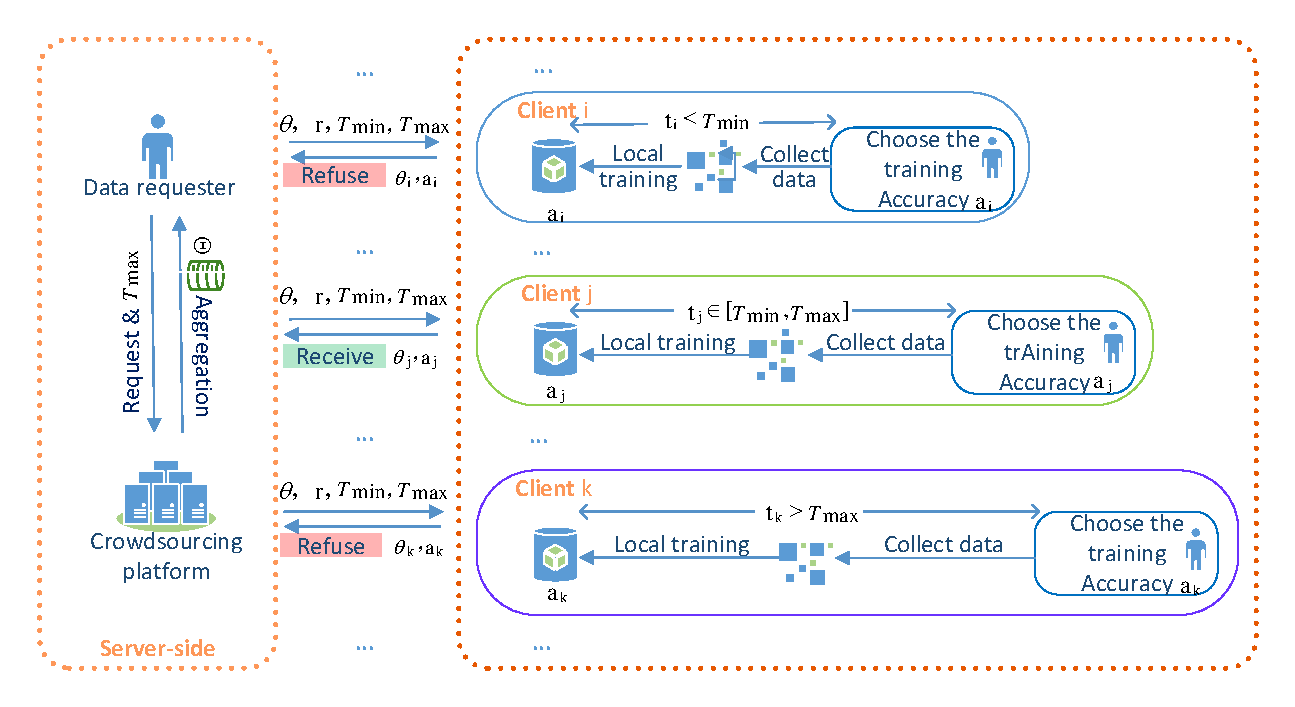
\includegraphics[width=5.4in]{TiFedCrowd framework.pdf}
	\caption{Framework of the Time-controlled incentive federated crowdsourcing (TiFedCrowd).}
	\label{fig:framework}
\end{figure}
\subsection{Incentive Mechanism: The Two-Stage Stackelberg Game}
In the proposed time-controlled incentive federated crowdsourcing model, the data requster reward clients who complete tasks within the specified time to achieve optimal local accuracy, thereby optimizing the global model. Simultaneously, upon receiving the rewards, rational clients will maximize their own profits respectively. We model such interaction scenario as a two-stage stackelberg game between a server (leader) and multiple clients(followers). In stage \uppercase\expandafter{\romannumeral2}, each client individually determines his/her own training accuracy with the announced reward to maximize profit. In stage \uppercase\expandafter{\romannumeral1}, the server decides on the reward rate for clients to maximize the net utility and train the high-quality global model.

\textbf{Stage \uppercase\expandafter{\romannumeral2} (Clients):} In the clients stage, the server will Initially announce the uniform reward rate $r>0$ and time interval $[T_{min},T_{max}]$ for the participating clients. Rationally, for a client $k$, the reward $v_k$ is related to the accuracy level $a_k$ of the local model $\theta_k$. Intuitively, the higher the local accuracy level, the greater the revenue:
\begin{equation}
	v_k = r\cdot a_k\cdot \mathbb{I}(\tau)
\end{equation}
where $\mathbb{I}(\tau)$ is an indicator function that returns $1$ if the condition $\tau$ is true and $0$ otherwise. Only if the completion time $t_k$ meets condition $\tau: t_k\in[T_{min},T_{max}]$ will the model $\theta_k$ be received by the server and the reward $v_k$ be allocated. We refer to clients whose models are successfully accepted by the server as valid participants. Then a rational worker will try to collect data to train local model for high accuracy within the time limit for maximizing the revenue. 

However, training on local data for a defined accuracy level to improve the global model inevitably incurs a cost for the clients, mainly the computation cost $c_k^{comp}$ and the communication cost $c_k^{comm}$ included:
\begin{equation}
	c_k^{comp} + c_k^{comm} = c_k
\end{equation}
where $c_k$ denotes the total cost of client $K$'s participation. The the computation cost $c_k^{comp}$ is relevant to the number of iterations for training the local model $\theta_k$ to the aim accuracy $a_k$. According to the relationship between iterations and accuracy in the local model training described in \citep{pandey2020crowdsourcing}, the computation cost of client $k$ is defined as
\begin{equation}
	c_k^{comp} = \gamma_k\cdot \log(\frac{1}{1-a_k})
\end{equation}
where $\gamma_k>0$ is a parameter choice of client $k$ that depends on the local subproblem whose data size and condition number. Therefore, the more iterations, the more computing resources the client spends.

The communication cost is related to the size of the model parameters and incurred when the client interacts with server for the model update. Since the to-be-trained model is published uniformly by the server, the total communication cost is the same for all clients:
\begin{equation}
	c_k^{comm} = \lambda\cdot\xi
\end{equation}
where $\lambda$ is a constant coefficient and $\xi$ represents the size of the model parameter.

Combined with the reward (1) and cost (2) of the client, we define the client utility model for the valid participant as:
\begin{equation}
	u_k = r\cdot a_k - c_k, \quad only\,\: if\quad\mathbb{I}(\tau) = 1
\end{equation}
\textbf{Stage \uppercase\expandafter{\romannumeral1} (Server):} In the server stage of the game, the server can evaluate the optimal reward rate $r^\ast$ to maximize its net utility according to the response of valid participants. Let $\zeta$ be the number of valid participants:
\begin{equation}
	\zeta = \sum_{k=1}^n\mathbb{I}(\tau)
\end{equation}
The server utility model can be defined in relation to the maximum completion time of valid participants and the final model performance achieved with average local accuracy level:
\begin{equation}
	U = \frac{1}{\zeta}\cdot \sum_{k=1}^n(\alpha\cdot a_k\cdot \mathbb{I}(\tau)) + \beta\cdot(T_{max}-\max_{\mathbb{I}(\tau)=1,1\le k\le n}t_k) - \sum_{k=1}^n(r\cdot a_k\cdot \mathbb{I}(\tau))
\end{equation}
where $\alpha > 0$ and $\beta \ge 0$ (default $\beta = 0$, and $\beta > 0$ only makes sense in instant crowdsourcing.) are system parameters, and $\sum_{k=1}^n(r\cdot a_k\cdot \mathbb{I}(\tau))$ is the cost totally spent for incentivizing clients to validly participate in federated crowdsourcing.
\subsection{Stackelberg-equilibrium}
In this subsection, we will find the optimal solution to maximize the utility of clients and server by deducing the Stackelberg-equilibrium. 

Defintion 1. Stackelberg-equilibrium. For any values of $r$ and $\bm{a}$, $(r^\ast,\bm{a}^\ast)$ is a Stackelberg-equilibrium if  it satisfies the following conditions:
\begin{equation}
	U(r^\ast,\bm{a}^\ast) \ge U(r,\bm{a}^\ast)
\end{equation}	
\begin{equation}
	u_k(r^\ast,a_k^\ast) \ge u_k(r^\ast,a_k),\, \forall k \in \bm{\mathcal{N}}
\end{equation}	

To find the equilibrium of the clients stage game, we take the first derivative of $u_k(r,a_k)$ with respect to $a_k$:
\begin{equation}
	\frac{\partial u_k(r,a_k)}{\partial a_k} = r-\frac{\gamma_k}{1-a_k}
\end{equation}	

Setting $\frac{\partial u_k(r,a_k)}{\partial a_k} = 0$, we have
\begin{equation}
	a_k^\ast = 1 - \frac{\gamma_k}{r}
\end{equation}	

Then, we take the second derivative of $u_k(r,a_k)$ with respect to $a_k$:
\begin{equation}
	\frac{\partial^2 u_k(r,a_k)}{\partial a_k^2} = - \frac{\gamma_k}{(1-a_k)^2} < 0
\end{equation}	

Hence, We derive and prove that $a_k^\ast = 1 - \frac{\gamma_k}{r}$ is the global optimal response accuracy of the client and is unique.

Since $0<a_k^\ast<1$, we can derive the value range of the reward rate $r$:
\begin{equation}
	0 < a_k^\ast = 1 - \frac{\gamma_k}{r} < 1\quad
	\Leftrightarrow\quad r > \gamma_k
\end{equation}	

Based on the above derivations for clients (followers), as the leader in the game, the server can deduce the unique Stackelberg-equilibrium among valid participants for any reward rate $r>\gamma_k$. Accordingly, the server can choose the optimal reward rate $r^\ast$ to maximize its net utility. Based upon the sets of the completion time $\bm{t}^\ast$ and the optinum response accuracy $\bm{a}^\ast$, the server utility model is defined as:
\begin{equation}
	U(r,\bm{a}^\ast) = \frac{1}{\zeta}\cdot \sum_{k=1}^n(\alpha\cdot a_k^\ast\cdot \mathbb{I}(\tau)) + \beta\cdot(T_{max}-\max_{\mathbb{I}(\tau)=1,1\le k\le n}t_k^\ast) - \sum_{k=1}^n(r\cdot a_k^\ast\cdot \mathbb{I}(\tau))
\end{equation}

Taking the first derivative of $U(r,\bm{a}^\ast)$ with respect to $r$, we get:
\begin{equation}
	\begin{aligned}
		\frac{\partial U(r,\bm{a}^\ast)}{\partial r} &= \frac{1}{\zeta}\cdot \sum_{k=1}^n(\alpha\cdot \frac{\partial a_k^\ast}{\partial r}\cdot \mathbb{I}(\tau)) - \sum_{k=1}^n(r\cdot \frac{\partial a_k^\ast}{\partial r}\ast\cdot \mathbb{I}(\tau)) - \sum_{k=1}^n(a_k^\ast\cdot \mathbb{I}(\tau))\\
		&= \frac{\alpha}{\zeta\cdot r^2}\cdot\sum_{k=1}^n(\gamma_k\cdot\mathbb{I}(\tau))-\zeta
	\end{aligned}
\end{equation}

Setting $\frac{\partial U(r,\bm{a}^\ast)}{\partial r} = 0$, we have:
\begin{equation}
	r^\ast =\frac{1}{\zeta}\cdot\sqrt{\sum_{k=1}^n(\gamma_k\cdot\mathbb{I}(\tau))}
\end{equation}	

The second derivative of $u_k(r,a_k)$ with respect to $a_k$ is:
\begin{equation}
	\frac{\partial^2 U(r,\bm{a}^\ast)}{\partial r^2} = - \frac{2\cdot\alpha}{\zeta\cdot r^3}\cdot\sum_{k=1}^n(\gamma_k\cdot\mathbb{I}(\tau)) < 0
\end{equation}	

Therefore, It is proved that $r^\ast = \frac{1}{\zeta}\cdot\sqrt{\sum_{k=1}^n(\gamma_k\cdot\mathbb{I}(\tau))}$ is the global optimal reward rate and unique. 

Ultimately, we find the unique Stackelberg-equilibrium of the game.
\subsection{Algorithm}
The pseudo-code of TiFedCrowd is shown in Algorithm~\ref{Algo1}. Lines 2-13 is the prodecure at server and lines 15-19 is at clients. Exactly, the process of the server-side includs the following 4 steps: estimate the minimum completion time (line 2), calculate the optimum response accuracy level at the given reward rate for each valid participant (lines 3-8), compute the optimum reward rate and announce it to clients, then wait until the deadline for them to complete the task (lines 10-12), receive the updated models and return the aggregated global model (lines 13).
The process of the client includes the following 3 steps: receive
the task completion time interval and the declared reward rate from the server (line 15), determine the optimum model training accuracy level and training to achieve it witnin the specified time interval (lines 17-18), and send the trained local model to server (line 19). 

\begin{algorithm}[H]
	\caption{\underline {Ti}me-controlled incentive \underline{Fed}erated \underline{Crowd}sourcing (TiFedCrowd)}
	\label{Algo1}
	\begin{algorithmic}[1]
		\REQUIRE clients $\bm{\mathcal{N}} = \{1,2,\dots,n\}$; local data samples sets ${D_k}_{k=1}^n$; computation
		parameters ${\gamma_k}_{k=1}^n$; size of the published model $\xi$;  system parameters $\alpha$ and $\beta$; completion deadline $T_{max}$.
		\ENSURE  global model $\Theta$.
		\STATE Procedure at the Server:
		\STATE Estimate the minimum completion time $T_{min}$.
		\FOR{all clients $k = 1 \to n$ in parallel}
		\IF {completion time $t_k\in[T_{min},T_{max}]$}
		\STATE Compute the client $k$’s utility $u_k$ at the given reward rates $r$ via Eq. (5).
		\STATE Calculate the optimal response accuracy level $a_k^\ast$ via Eq. (11).
		\ENDIF
		\ENDFOR
		\STATE Compute the task server’s utility via Eq. (14).
		\STATE Choose the optimum reward rate $r^\ast$ via Eq. (16), then announce it to all clients.
		\STATE Wait until time $T_{max}$ for clients to complete the data collection and model training.
		\STATE Receive the updated models ${\theta_k}_{k=1}^n$ and send the rewards to valid participants based on their accuracy level.
		\STATE return the aggregated global model $\Theta$.
		\STATE Procedure at the Client $k$:
		\STATE Receive the time interval $[T_{min},T_{max}]$ and the reward rate $r$.
		\STATE Compute the client utility $u_k$ via Eq. (5).
		\STATE Determine the training accuracy level $a_k^\ast$
		to solve the local subproblem via Eq. (11).
		\STATE Collect the required data and train local model for attaining the accuracy level $a_k^\ast$ within the time interval $[T_{min},T_{max}]$.
		\STATE Upload the trained local model $\theta_k$ to the server.
	\end{algorithmic}
\end{algorithm}
\section{Experiments} \label{sec:exp}
\section{Conclusion} \label{sec:con}

\bibliography{ref,reference1}
\end{document}
